\documentclass[..]{subfiles}


\begin{document}

\chapter{Computation Model}\label{chap:model}

In the current chapter a formal model will be described that can be classified using the concepts explained in Chapter \ref{chap:previous}. This model is a personal take on \cite{canetti2001universally} which is the model used in the article this work is mainly based on \cite{garay2015bitcoin}.


% \section{Objective}
%
% The objective of the described model is to create a general enough frame to accommodate 


\section{Model Definition}

A protocol is a computer program, intended to be executed by a set of computational entities or \textit{parties} with the ability to communicate between them. A protocol execution is a set of interacting computing elements, each running the protocol on its own input and taking its own random choices. The \textit{adversary} noted with $\mathcal{A}$, is a computational entity that controls a subset of the parties and has some kind of control over the communication network. It represents a malicious entity trying to prevent parties from behaving correctly in terms of some protocol properties or the protocol objective itself. The \textit{environment}, noted by $\mathcal{Z}$, represents any external external condition to the current protocol like other protocol and their adversaries, human users, etc. The environment is allowed to interact with the adversary and the rest of the parties at any point of the execution. All parties interact until each one generates a local output. The concatenation of the local outputs of the adversary and all parties is called the \textit{global output}.


\subsection{Interactive Turing Machines}

In order to model the computational objects that parties represent an extension of the traditional Turing machines will be used. \textit{Interactive Turing Machines} are an extension on the standard Turing machine created to capture the casuistry of a distributed algorithm, namely a protocol. 

\begin{definition}
	\normalfont
	An \textit{interactive Turing machine(ITM)} $\mu$ is a Turing machine with the following augmentations:
	\paragraph{New Data Structures:}
	\begin{itemize}
		\item \texttt{Identity tape}: This tape is ``read only''. Its content is interpreted as two strings. The first string is a description of the program run in the on $\mu$, i.e, its state transition function and initial tape contents. This is called $\mu$ code. The second string is an identifier called \textit{identity} of $\mu$. The code and the identity are called the \textit{extended identity} of $\mu$.

		\item \texttt{Outgoing message tape}: This tape holds the current outgoing message along with enough addressing information for message delivery.

		\item \texttt{Input tape}: This tape is ``read only''. This tape represents incoming messages. 
	\end{itemize}

	\paragraph{New Instructions:}
	\begin{itemize}
		\item \texttt{External write}: The effect of this instruction is that the message currently written on the outgoing message tape is possibly written to the input tape of the machine with the identity specified in the outgoing message tape.
		\item \texttt{Read next message:} The effect of this instruction is that the reading head jumps to the beginning of the next message on that tape. In order to implement this instruction it can be supposed that each instruction ends with a special character.
	\end{itemize}
\end{definition}

\begin{definition}
	\normalfont
	A \textit{configuration} of an ITM $\mu$ consists of the contents of all tapes, as well as the current state and the location of the head in each tape. A configuration is active if the activation tape is set to 1, else it is inactive.
\end{definition}

Each party on the system will be modeled as ITM, including the ones controlled by the adversary $\mathcal{A}$. In the \textit{bitcoin backbone protocol} $\mathcal{A}$ will have some communication advantages over the honest of the parties. In order to model this situation a control program, noted $C$, has to be introduced. $C:\{0,1\}* \rightarrow \{allow, deny \}$ takes any configuration of an ITM and an ITM identity and returns a value meaning the function has or not permission to directly communicate with ITM. Now, communication between parties can be formally defined.

\paragraph{Communication}
Communication between parties is based on the \texttt{External write}. Let $M = (\mu, id)$ denote the ITM which executes instruction \texttt{External write}. Then the current contents of the outgoing message is interpreted as a sequence of tuples:
$$(id, id', r, m)$$
Where $id$ is the machine's $id$, $id'$ is an ITM identity, $r$ is the \texttt{reveal-sender-id} flag and $m \in \{0, 1\}*$ is the \texttt{message}. Iteratively over the sequence of tuples, consider the output of function $C$ when given $(id, id', r, m)$ as input. If this is $disallow$, then the instruction is not carried out and the calling machine is halted. If $C$ outputs $allow$, then if an ITM $M'$ with identifier $id'$ exists on the system then message $m$ is written to the input tape of $M'$. If the \texttt{reveal-sender-id} flag is set, then the identity of $M$ is also written to the input tape of $M'$. The control program $C$ may output $disallow$ in several cases like the $id$ written on the message not coinciding with the real machine address(which can't be changed since the \texttt{identity tape} is read only) or if the sender machine does not have permission to input a communicate with the addressee machine.

\begin{figure}[H]
	\begin{center}
		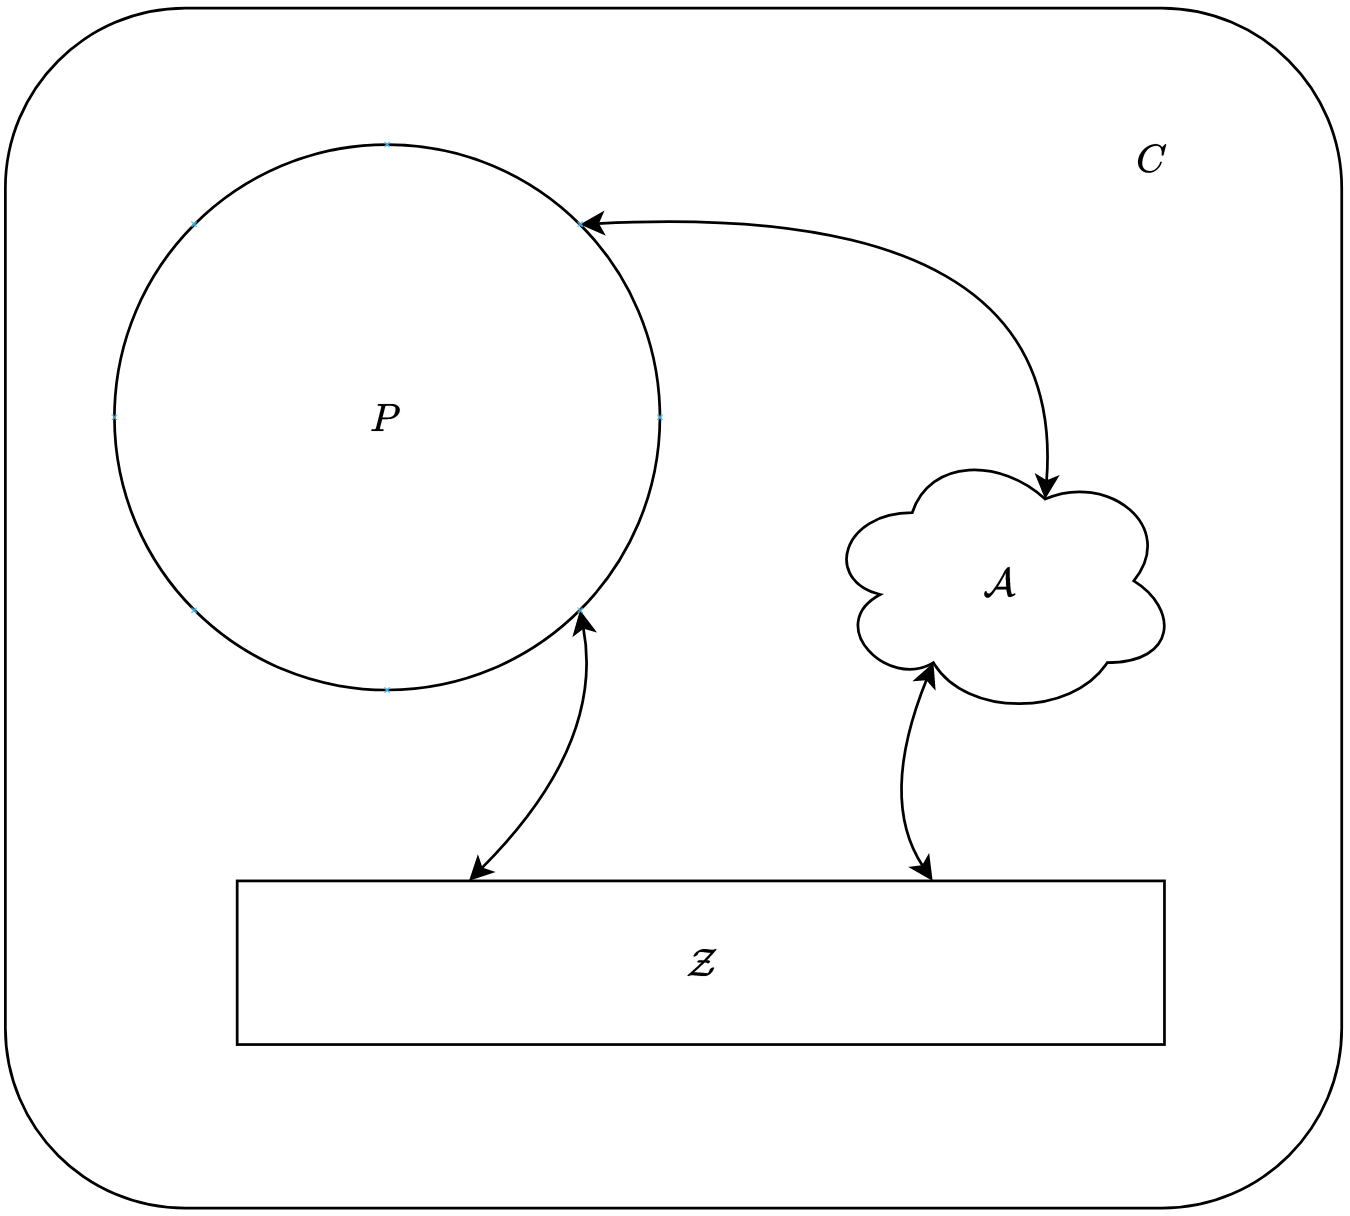
\includegraphics[width=0.58\textwidth]{figures/model.png}
	\end{center}
	\caption{Model sketch}
	\label{fig:model_sketch}
\end{figure}


\paragraph{Polynomial Time ITMs}

A Turing machine $\mu$ is said to be $T$-bounded if, given any input of length $n$, $\mu$ halts within at most $T(n)$ steps. This guarantees that an execution of a system of ITMs completes in bounded time. An interactive Turing machine $\mu$ is said to be $T$-bounded if, given any input of length $n$, $\mu$ halts within at most $T(n) + T(m) - T(m')$ steps where $m$ is the number of received messages during its execution and $m'$ is the number of sent messages.

\subsection{Services}

During the definition of the \textit{Bitcoin backbone protocol} there will be a need to use certain certain processes that are are different in their purpose and scope from the protocol parties. A \textit{function} will be the equivalent of a mathematical function, it maps inputs to outputs. A \textit{functionality} is different from a function in the sense that it maintains a \texttt{state} that may be updated with each call. Last an \textit{oracle} is a functionality that has a random component to it. All of these entities will be modeled by ITMs each with a special identifier that allows parties in the system to identify and communicate with them. Since they are modeled by ITMs they will use function \texttt{Read next message} to read the next message in its input and tape, process it and write the pertinent output to the senders ITM which must have specified its $id$ and set $r=1$ in its message. By this mechanism it can be said that these services can be accessed in a concurrent manner. As stated these processes are not considered parties.


\subsection{Protocol execution}

A \textit{system of ITMs} is a pair $S = \langle Z, C\rangle$ where $Z$ is an environment and $C$ is a control function. Parties and services have their code written in their identity tape but not their identity. The execution of a system $S = \langle Z, C\rangle$ goes as follows. First, the control program writes a unique identity for each party in $Z$ and each service. Next $C$ sends the start signal to all parties. Parties execute their code and interchange messages following the rules coded in $C$ until they obtain an output, then they execute a special halt instruction which writes their output on $C$ and halts the machine. When all parties have written their respective output on the input tape of $C$ the initial machine writes a final message in $Z$ and halts. Execution is ended.



\end{document}

